\documentclass[10pt,a4paper]{article}
\usepackage{fontspec,polyglossia}\setmainlanguage{russian}\setmainfont{Times New Roman}
\usepackage{amsmath,amssymb,booktabs,tabularx,graphicx}\usepackage[margin=17mm]{geometry}
\usepackage[hidelinks]{hyperref}\usepackage{titlesec}\titleformat{\section}{\large\bfseries}{}{0pt}{}
\titlespacing*{\section}{0pt}{8pt}{4pt}\setlength{\parindent}{0pt}\setlength{\parskip}{4pt}\setlength{\emergencystretch}{3em}
\begin{document}
{\Large\bfseries Развитие Walker2d-сеттинга: динамика MG во время обучения}\par\medskip

\section*{Идея}

В предыдущем опыте PPO обучался со штрафом за изменение среднего действия политики. Поэтому контролируемое упрощение относится прежде всего к управляющему логу. Здесь проверяется не только финальная политика, но и пять промежуточных чекпоинтов: одинаковый ли сигнал MG появляется постепенно вместе с уменьшением сложности действий.

Обозначим $a_t$ как шестимерную команду политики. Вмешательство добавляет к PPO-loss штраф на квадрат первой разности среднего действия. Независимые показатели:

\[
J_1=\frac{1}{6T}\sum_t\|a_t-a_{t-1}\|^2,
\qquad
J_2=\frac{1}{6T}\sum_t\|a_t-2a_{t-1}+a_{t-2}\|^2.
\]

MG пересчитывался по скалярному логу $\|a_t\|$ с теми же параметрами, что в основном опыте: окно 2048, задержка 8, 20 координат вложения и 20 соседей. Значения сравниваются с обычным PPO на том же сиде и том же тестовом сбросе.

\section*{Как измерялось}

Использованы уже обученные пары сидов 221--225. Новых обучений не проводилось. Для каждого сида и каждого варианта взят чекпоинт после 0, 262144, 524288, 786432 и 1048576 переходов. На каждом чекпоинте записана одна траектория длиной 4096 шагов из фиксированного тестового сброса 62001. MG считался по последнему окну 2048 шагов.

На одном промежуточном чекпоинте сглаженная политика упала. Эта запись не заменялась нулём и исключена из медианы соответствующего этапа; поэтому для 786432 переходов имеются 4 пригодные пары для MG, J1 и J2. На остальных этапах доступны все 5 пар.

\section*{Результаты}

\begin{center}\small
\begin{tabularx}{\linewidth}{l>{\raggedright\arraybackslash}X>{\raggedright\arraybackslash}X>{\raggedright\arraybackslash}X>{\raggedright\arraybackslash}X}
\toprule
Переходы & MG: норма действия & J1 & J2 & Пригодных пар \\
\midrule
0 & 1.000 & 1.000 & 1.000 & 5 \\
262144 & 0.778 & 0.417 & 0.235 & 5 \\
524288 & 0.766 & 0.317 & 0.162 & 5 \\
786432 & 0.824 & 0.275 & 0.133 & 4 \\
1048576 & 0.898 & 0.318 & 0.165 & 5 \\
\bottomrule\end{tabularx}\end{center}

\begin{center}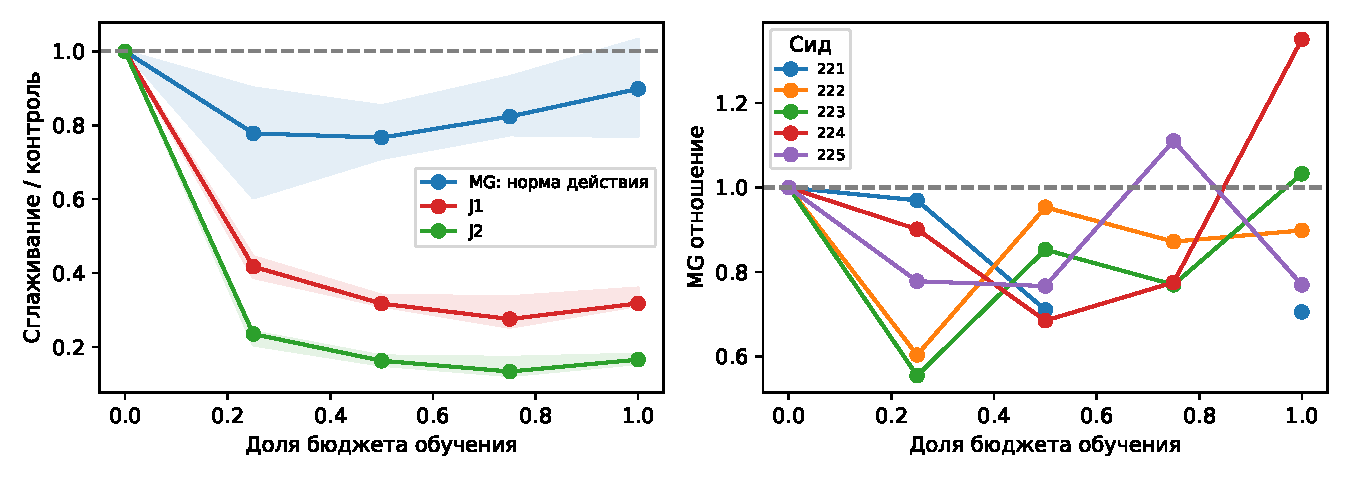
\includegraphics[width=\linewidth,height=.32\textheight,keepaspectratio]{checkpoint_timecourse.pdf}\end{center}

После первых 262144 переходов MG уже снижается до 0.78 от контроля. Минимум медианного отношения наблюдается около 524288 переходов --- 0.77. Затем MG частично возвращается к единице, хотя J1 и J2 остаются существенно ниже контроля. Поэтому MG реагирует на упрощение лога, но его значение не обязано монотонно следовать штрафу или плавности.

По отдельным сидам финальное отношение MG равно 0.705, 0.898, 1.033, 1.351 и 0.769. Это показывает, что медианный положительный результат не означает одинаковое поведение каждой пары. Временная проверка также выявляет падение на одном промежуточном чекпоинте; такие события нужно сохранять, а не скрывать усреднением.

\section*{Что добавляет этот анализ}

Он переводит эксперимент из финального сравнения в более содержательный сценарий мониторинга обучения:

1. на старте контроль и сглаженная политика совпадают, поэтому отношение MG равно 1;
2. после начала регуляризации MG управляющего лога снижается одновременно с J1 и J2;
3. на поздних этапах J1 и J2 могут оставаться низкими, а MG частично возвращаться, то есть это разные диагностические величины;
4. MG по одному управляющему скаляру не следует переносить на всю физическую траекторию Walker2d.

Практически это поддерживает формулировку: MG может быть дешёвым монитором изменения сложности конкретного лога во время обучения. Для вывода об упрощении полной динамики нужны дополнительные наблюдаемые величины и контроль падений.

\section*{Следующий вариант постановки}

Следующий эксперимент следует строить как факторный тест коэффициента регуляризации на одном и том же наборе сидов: $\lambda\in\{0,0.25,1,4\}$. Для каждого значения заранее фиксируются J1, J2, MG нормы действия и MG отдельных каналов. Основной анализ должен проверять не только знак финального отношения, но и кривую по чекпоинтам, а коэффициент нельзя выбирать по MG после просмотра результатов.

Текущий результат не является доказательством уменьшения активной размерности полной Walker2d-системы. Он показывает более узкое и воспроизводимое утверждение: при явно заданном сглаживании управляющих команд MG на агрегированном управляющем логе обычно обнаруживает происходящее упрощение, хотя сигнал зависит от времени и конкретного сида.
\end{document}